\section{Das Wie der Umsetzung}
\label{sec-5}
\fbox{
\parbox{\linewidth}{
	\textit{Ziel des Kapitels:}\\
	Umsetzung erläutern: Wie wurde die Lösungsidee umgesetzt?\\[6px]
	\textit{Inhalte:}
	\begin{itemize}
		\item Welche Darstellungen wurden gewählt?
		\item Wie wurde die Interaktion gestaltet?
	\end{itemize}
}}
\subsection{Architektur der Anwendung}
%TODO Komponentendiagramm erstellen
\begin{itemize}
	\item Blender, Unity, Vuforia
	\item Übersicht Komponenten und Zusammenspiel
\end{itemize}

\textbf{Client-Server Datenübertragung}
\begin{itemize}
	\item HoloLens erfragt Daten vom Server über HTTP GET-Requests
	\item Asynchrone Anfragen, so wird Render-Prozess nicht blockiert
	\item Server nimmt Request entgegen und hält eine Antwort solange zurück, bis er einen neuen Wert vom Arduino erhält, der der HoloLens noch nicht bekannt ist und von vorherigen Werten signifikant abweicht
	\item Dadurch kommen neue Daten sehr schnell bei der HoloLens an, der Nutzer sieht die Änderungen auf der Brille sofort, wenn er Änderungen an der Spannungsquelle vornimmt
	\item Dadurch wird zeitliche Einbettung und Kontinuität erreicht
	\item Dabei wird jedoch kein unnötiger Traffic erzeugt, wenn es keine Änderungen gibt
	\item Das spart Ressourcen
\end{itemize}
\begin{figure}[h!]
	\centering
	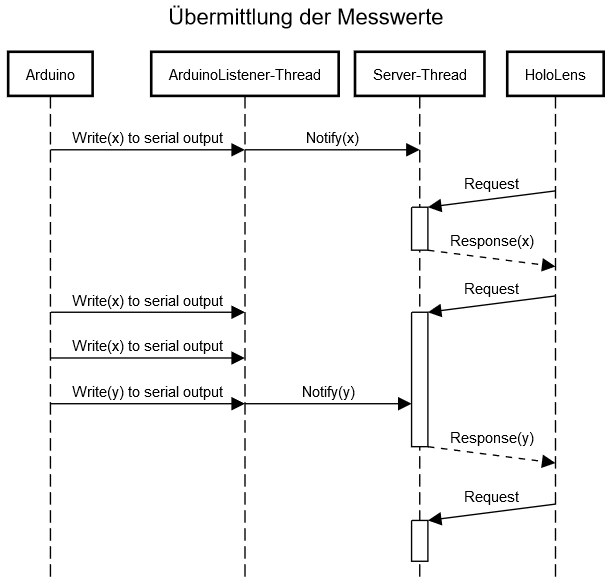
\includegraphics[width=1\textwidth]{images/Sequenzdiagramm.png}
	\caption{Sequenzdiagramm Kommunikation}
	\label{img:Sequenzdiagramm}
\end{figure}

\subsection{Darstellung}
\textbf{Felddarstellung}
\begin{itemize}
	\item Min Force 3, Max 80, konsistent bei allen Darstellungen
	\item Fading von 3-10
	\item Pfeile und Linien mit ca. 3,5 cm Durchmesser
\end{itemize}
Feldlinien
\begin{itemize}
	\item Mindestens 4 (2x2) (notwendig um Homogenität zu erkennen)
	\item Maximal 16 (4x4)
	\item Zylindrischer Ausschnitt gewählt mit $r=2/3 * R = 10 cm$
	\item Abstandsformel: 
	\item Dargestellte Größe: Flussdichte
\end{itemize}
Vektoren
\begin{itemize}
	\item Mindestens 8 (2x2x2) (notwendig um Homogenität zu erkennen)
	\item Maximal ???
	\item Gewählte Rasterisierung:
	\item Längenformel:
\end{itemize}

\textbf{Occlusion Berechnung}
\begin{itemize}
	\item Für Verdeckung werden maßstabsgetreu nachmodellierte, virtuelle Objekte verwendet
	\item 3D Mesh in Blender erstellt, 2mm größer als echte Objekte für Spielraum
	\item Objekte werden möglichst genau über reale gelegt
	\item Rendering erfolgt ausschließlich in den Z-Puffer, dadurch sind die realen Objekte sichtbar, die virtuellen verdecken jedoch dahinterliegende, vrituelle Objekte
	\item Das Near Clipping Plane muss dafür jedoch sehr nah am Kameraursprung liegen, andernfalls würden weiter entfernte, virtuelle Objekte plötzlich doch vor realen Objekten angezeigt werden, sobald letztere zu nah sind und das Clipping die Objekte vom Rendering ausschließt
\end{itemize}

\textbf{Near Plane Fading}
\begin{itemize}
	\item MRTK Standard Shader implementiert Fade To Black
	\item Shader auf Fade to transparent abgeändert
	\item Lineares Fading überall genutzt
\end{itemize}

\textbf{Kompass-Linien und Strom-Pfeile}
\begin{itemize}
	\item Darstellungen über 2D-Linien mit Unity's LineRenderer
	\item Für gestrichelte Linien eine Textur mit einem weißen Kreis und transparentem Hintergrund, dabei wird die Skalierung mit Tiling auf die Länge der Linie angepasst
	\item Strom-Pfeile haben Bilboard-Verhalten, Maßgebend ist dabei die Vorwärtsrichtung ihres Transform.
	\item Fade-Away-Effekt verhindert zu steile Winkel, so sind immer die relevanten Pfeile sichtbar
\end{itemize}

\textbf{Textboxen}
\begin{itemize}
	\item Verwendung der im MRTK vorhandenen Schriftsätze
	\item Dunkelgrauer Hintergrund verbessert Lesbarkeit, da Text vor transparentem Grund vor einigen Hintergründen schwer zu lesen ist
	\item Dank leicht transparenter Hintergrund ist die Textbox nicht so dominant im Bild und die dahinterliegenden Objekte sind für den Nutzer noch sichtbar
	\item Umsetzung als 3D Objekt, damit wird Stabilisierung genutzt
\end{itemize}

\textbf{Weiteres}
\begin{itemize}
	\item Spracherkennung über eigens gewählte, englische Keywords, Erkennung durch Microsoft's built-in Spracherkennung
	\item Drag-and-Drop über MRTK HandDraggable 
\end{itemize}

\subsection{Interaktion}
\begin{itemize}
	\item Per Klick Geste zwischen verschiedenen Modi umschalten
	\item Per virtueller Tastatur Eingabe von numerischen Werten
	\item Per Keywords "Power on" und "Power off" Steuerung des Stromkreises
	\item Klick-Feedback durch Sound
	\item ...
\end{itemize}
